% File example.tex
% Contact: simonnet@ecole.ensicaen.fr
%
% version 1.0 (July 24, 2009)
% version 1.1 (September 3, 2009)
% add using of the optional command: \secondauthoraddr

\documentclass[10pt]{article}

% File icdp2009.sty
% Preamble that you have to include to use the template  

% July 24, 2009
% Contact: simonnet@ecole.ensicaen.fr


\usepackage[a4paper,textwidth=18cm,textheight=24cm,top=2.85cm, bottom=2.85cm, left=1.5cm, right=1.5cm]{geometry}

\usepackage{includes/icdp2009}

% left justified caption
\makeatletter
\long\def\@makecaption#1#2{%
\vskip\abovecaptionskip
\sbox\@tempboxa{#1. #2}%
\ifdim \wd\@tempboxa >\hsize
#1. #2\par
\else
\global \@minipagefalse
\hb@xt@\hsize{\box\@tempboxa\hfil}%
\fi
\vskip\belowcaptionskip}
\makeatother




%other package

% vectorial font
\usepackage{lmodern}

\usepackage{graphicx}
\usepackage{times}

\usepackage{textcomp}
\usepackage[justification=centering]{caption}

\begin{document}
\noindent

% This should produce references in the order they appear
\bibliographystyle{ieeetr}

\title{Automatically landmarks prediction on Beetle's pronotum}
%\title{An improvement on estimated landmarks of Beetle's pronotum}

\authorname{Le Van Linh$^{1,3}$, Beurton-Aimar Marie$^{1}$, Zemmari Akka$^1$, Parisey Nicolas$^2$}
\authoraddr{$^1$LaBRI - CNRS 5800 Bordeaux University, France, van-linh.le/beurton/zemmari@labri.fr}

%optional
\secondauthoraddr{$^2$IGEPP - INRA 1349, France, nparisey@rennes.inra.fr }
\thirdauthoraddr{$^3$ITDLU - Dalat University, Vietnam, linhlv@dlu.edu.vn}


\maketitle

\keywords
Landmarks, convolutional neural networks, fine-tuning, recogntion, procrustes.

\abstract
In recent years, deep learning is known as a good solution for the difficult problems in computer vision. It appears in many fields such as classification, recognition, face detection. In this paper, we propose a scenario to predict the landmarks on 2D images, specify beetle's head images. The proposed method includes two stages: firstly, the landmarks are estimated by applying convolutional neural network; then, the estimated landmarks are verified to increase the accuracy. The method experimented on a set of 293 images. The accuracy of the method is evaluated by calculating the distance in pixels between the coordinates of the predicted landmarks and manual landmarks which were provided by the biologists.

\section{Introduction}
Morphometry landmark (or point of interest) is an important feature in many biological investigations. It was usually used to analyze the forms of whole biological organs or organisms. The analysis is mainly based on the coordinates of the landmarks. The collecting of enough the number of landmarks can help the biologists make a good estimate about organisms. Depending on the problem, the number of landmarks may be more or less; besides, the location of landmarks can be located on the shape (border) or inside the object, \textit{for examples,} the landmarks on Drosophila wings have stayed on the veins of the wings but the landmarks on human ear can be located at the ear hole or inside. Recently, the landmarks were set manually by the biologist. This work is time-consuming and difficult to reproduce. Therefore, a method that proposes automatically the coordinates of landmarks could be a concern. 

Based on the characteristics of the images, the images can be divided into two groups: the images that we can easy to segment the objects in the image, called segmented images; and the images that we can go in tight when segment the objects, called un-segmented images. For that reason, the methods that used to identify the landmarks automatically may be divided into two groups too. For segmented images, identification of landmarks on the shape can be finished by applying the image processing techniques such as HOG\cite{•}, SIFT\cite{•}, .... But for un-segmented images, defining the landmarks become a challenge and the image processing techniques seem to be inappropriate. This article introduces a scenario for automatic detection of the landmarks on biological images, specific beetle's head images, called \textit{pronotum} images (Fig. \ref{figpronotum}). The method includes 2 stages: 1) the initially predicted landmarks are given by a convolutional neural network (CNN) \cite{•}; 2) the predicted landmarks which located in the shape of pronotum will be refined the location to increase the accuracy of coordinates. In the first stage, the main idea is design and train a CNN with a set of images and their manual landmarks. The dataset includes $293$ pronotum images and their manual landmarks which have been provided by the biologists. The images are presented in two dimensions and RGB color. After training, the trained network will be able to detect the initially predicted landmarks on the pronotum images. In the second stage, the predicted landmarks in the shape will be refined the coordinates by applying a Procrustes analysis\cite{•}. For each manual landmark, a model is generated as a specific. Then, it is used to refine the corresponding predicted landmarks.

\begin{figure}[htbp]
\centering
	\centerline{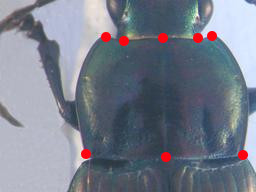
\includegraphics[scale=0.65]{images/pronotum}}
	\caption{An example of pronotum images and its manual landmarks}
	\label{figpronotum}
\end{figure}

In the next section, we present related works in domain automatically estimation landmarks on 2D images. In section 3, we present an overview about the stage that predict the initial automatically landmarks by applying CNN. The procedure apply to refine the predicted landmarks which provide by CNN will be presented in section 4. In the last section, we show all the experiments and analysing the results.

\section{Related works}
Landmarks or points of interest are one of the important characteristics in geometric morphometrics. Landmark studies have traditionally analyzed on 2D images. Depending on which situation was stayed (segmented or un-segmented images), setting landmarks must apply the different methods.

When segmentation can be applied, Lowe et al. \cite{•} have proposed a method to identify the key points in the 2D image. From the detected key points, the method is able to match two images. Palaniswamy et al. \cite{•} have applied probabilistic Hough Transform to automatically estimate the landmarks in images of Drosophila wings. Adrien et al. \cite{•} have extended Palaniswamy's method to detect landmarks automatically on beetles mandibles. Unfortunately, this method can not be applied to other parts of beetle that the segmentation has too many noises, such as pronotum images.

%It presents a learning method with multiple levels of representation of connected layers (convolutional neural network). Data representation is transform from a lower level to a higher level with many complex functions can be learned.
Recently years, machine learning is developing rapidly, specifically deep learning (CNN). It exists in most of the fields, especially in computer vision. We can finish a lot of difficult tasks with a deep convolution neural network such as classification \cite{•}, image recognition \cite{•}, speech recognition \cite{•} and language translation \cite{•}. Using CNN to determine landmarks on 2D images will produce good results and it may be a good solution for the un-segmented images. Yi Sun et al. \cite{•} have proposed a cascaded convolutional network to predict the key points on the human face. Zhang et al. \cite{•} optimizes facial landmarks detection with a set of related tasks such as head pose estimation, age estimation, .... Cintas et al. \cite{•} have introduced a network to predict the landmarks on human ear images. In the same context, we have applied CNN to predict the landmarks on pronotum images. The predicted landmarks then refined to increase the accuracy of coordinates.

\section{Automatic landmarks by using CNN}
\subsection{Network architecture}

\subsection{Data processing}
Figures and tables should be centred in the column, numbered
consecutively throughout the text, and each should have a
caption underneath it (see for example Table 1). Care should
be taken that the lettering is not too small. All figures and
tables should be included in the electronic versions of the full
paper. We cannot guarantee that any printed version of the
proceedings will use colour.


\begin{figure}[h]
\centering

\includegraphics[width=1.5cm]{images/fig1}
\caption{\label{tab1}This is an example of a figure caption.} 
\end{figure}


\begin{table}[h]
\begin{center}

\begin{tabular}{c}
nn!1 \\
2 \\
31 \\
6 \\
\end{tabular}
\end{center}
\caption{\label{tab1}This is an example of a table caption.}
\end{table}

Equations should be typed within the text, centred, and should
be numbered consecutively throughout the text. They should
be referred to in the text as Equation (n). Their numbers
should be typed in parentheses, flush right, as in the following
example.
\begin{equation}
	    PA + A'P - PBR^{-1}B'P + Q  =  0 \enspace.
\end{equation}
\subsection{Training and experiments}

\section{Improving the predicted landmarks}
The PDF format will be the final format under which the
papers will appear in the Proceedings. Therefore you are
required to submit your paper as PDF document. If this is not
possible, Postscript format is also accepted as long as no fonts
other than the recommended fonts are used.

You can use any of the popular free LaTeX editors (e.g. Kile).

\section{Results}
The submission process for ICPRS 2018 should be done on
line at http://www.icprs.org

A PDF version of your final paper is required. It should
be expected that after your submission, your paper is
published directly from the file you send without any further
proofreading. Therefore, it is advisable for the authors to
print a hard copy of their final version and read it carefully.

\section{Conclusions}
The list of references should be ordered in the same order as
first cited in the text. All references should be cited in the
text, and using square brackets such as \cite{ref01} and \cite{ref01,ref02}. We
recommend the use of IEEE Transactions style for references.

\section*{Acknowledgements}
The acknowledgement for funding organisations etc. should
be placed in a separate section at the end of the text.



Thank you for your cooperation in complying with these
instructions.


\bibliography{IEEEabrv,includes/icdp2009}


\end{document}
